% =====================================================
%  Domain Event & DDD — Full Slide Deck
% =====================================================
\documentclass{beamer}
\usetheme{Madrid}

% ----------- Packages ----------
\usepackage[T1]{fontenc}
\usepackage[utf8]{inputenc}
\usepackage{xcolor}
\usepackage{listings}
\usepackage{graphicx}
\usepackage{hyperref}
\hypersetup{colorlinks,linkcolor=black,urlcolor=blue}

\usepackage{pgfpages}
\usepackage{tikz}
\usetikzlibrary{positioning}
\setbeameroption{show notes}

% ----------- Layout ----------

\AtBeginSection[]{
  \begin{frame}
    \vfill
    \begin{center}
        \usebeamercolor{title}
        {\Huge \insertsection}
    \end{center}
    \vfill
  \end{frame}
}


% ----------- Code Listing Style ----------
\lstset{
  language=Java,
  basicstyle=\ttfamily\scriptsize,
  keywordstyle=\bfseries\color{blue},
  commentstyle=\itshape\color{gray},
  stringstyle=\color{purple},
  numbers=left, numberstyle=\tiny\color{gray}, numbersep=5pt,
  breaklines=true, showstringspaces=false,
  columns=flexible, tabsize=2,
  frame=single, framerule=0pt,
  backgroundcolor=\color{gray!6}
}

% ----------- Project Information ----------
\title[Domain Event]{Implementing Domain-Driven Design \\ Domain Event}

% ======================================================
\begin{document}
% ------------------------------------------------------

\begin{frame}
  \titlepage
\end{frame}

\begin{frame}{Overview}
    \scriptsize
    \tableofcontents[hideallsubsections]
\end{frame}

\section{1. The Concept of Events \& "When/Why"}

\begin{frame}{1-1. Definition in One Sentence}
  \begin{block}{Domain Event}
    A "fact" that has occurred in the business domain and is worthy of notice, preserved as an object.
  \end{block}

  \begin{itemize}
    \item<1-> Keywords: \textbf{Happened (past tense)}, \textbf{Business Significance}
    \item<2-> Can be \textbf{replayed} / \textbf{propagated}
  \end{itemize}
\end{frame}

\begin{frame}{1-2. Why Use Events?}
  \tiny
  \begin{tabular}{|p{2.5cm}|p{4cm}|p{4cm}|}
    \hline
    \textbf{Scenario} & \textbf{Without Events...} & \textbf{With Events...} \\
    \hline
    Async Integration (Other systems need to know when a user pays) & Direct RPC call → May hang if the other system is down & Publish `PaymentConfirmed` event → Queued in MQ, consumer handles it later \\
    \hline
    One Tx, one Aggregate & Updating two Aggregates synchronously → Breaks consistency or requires XA & Modify A first → Publish event → Handler opens new Tx to modify B \\
    \hline
    Replacing Batch Jobs & Scan DB at night for "state changes" & Event is pushed to a service immediately, logic is spread out \\
    \hline
  \end{tabular}
\end{frame}

\begin{frame}{1-3. How to Identify an Event?}
  When talking with a Domain Expert, these phrases are red flags:
  \begin{itemize}
    \item<1-> \textbf{"When... happens"}: \textit{“When an order ships, send the customer a mail.”}
    \item<2-> \textbf{"If... then..."}: \textit{“If the balance drops below zero, freeze the account.”}
    \item<3-> \textbf{"Notify me..." / "Tell me..."}: \textit{“Notify finance if a refund exceeds \$10,000.”}
  \end{itemize}
  \vfill
  \begin{alertblock}{}
    → This indicates a business rule needs to react to "something happening," which is a strong candidate for an event.
  \end{alertblock}
\end{frame}

\begin{frame}{1-4. Events ≠ CRUD Logs}
  \begin{itemize}
    \item It's \textbf{not} about calling it `RowInsertedEvent` just because a row was added.
    \item It must be at the \textbf{business semantic level}—"UserRegistered," "InventoryDeducted"—to be valuable.
  \end{itemize}
\end{frame}

\begin{frame}[fragile]{1-5. Minimal Java Event Interface}
  \begin{lstlisting}
// Every event must implement this interface
public interface DomainEvent {
    Date occurredOn();
}

// Example of a concrete event
public class UserRegistered implements DomainEvent {
    private final String userId;
    private final String email;
    private final Date occurredOn;

    public UserRegistered(String userId, String email) {
        this.userId = userId;
        this.email = email;
        this.occurredOn = new Date();
    }

    @Override
    public Date occurredOn() {
        return this.occurredOn;
    }
    
    // Other getters...
}
  \end{lstlisting}
\end{frame}

\begin{frame}{✅ A Small Exercise For You}
  \begin{enumerate}
    \item Think about your current system. \textbf{What business actions are named in the past tense}?
    \item List them out. Don't worry about code yet, just confirm the semantics.
  \end{enumerate}
\end{frame}


\section{2. How to Name and Model Events}

\begin{frame}[fragile]{2-1. Event Name: Past Tense + Ubiquitous Language}
  \begin{enumerate}
    \item \textbf{Source = Command}
      \begin{itemize}
        \item In the Scrum AgilePM example, the `BacklogItem` aggregate has an action:
        \begin{lstlisting}[language=Java]
backLogItem.commitTo(aSprint);
        \end{lstlisting}
        \item This "action" is the \textbf{cause} of the event.
      \end{itemize}
    \item<2-> \textbf{Name = Past Tense of the Cause}
      \begin{itemize}
        \item Because `commitTo()` has completed, the event is named `BacklogItemCommitted`.
      \end{itemize}
  \end{enumerate}
  \begin{alertblock}<3->{Principle}
    The name alone should make it clear that "this has happened" and fully align with the Bounded Context's \textbf{Ubiquitous Language}.
  \end{alertblock}
\end{frame}

\begin{frame}[fragile]{2-2. Minimal Domain Interface: \texttt{DomainEvent}}
  \lstset{language=Java} % Set language for this frame
  The book first defines a very thin interface that all events must implement:
  \begin{lstlisting}
package com.saasovation.agilepm.domain.model;

import java.util.Date;

public interface DomainEvent {
    Date occurredOn();
}
  \end{lstlisting}
  \begin{itemize}
    \item Has only one responsibility: return the event's occurrence time via `occurredOn()`.
    \item Keeping it minimal ensures events remain \textit{lightweight} and easy to serialize.
  \end{itemize}
\end{frame}

\begin{frame}[fragile]{2-3. Event Class \texttt{BacklogItemCommitted}}
    \lstset{language=Java, basicstyle=\ttfamily\tiny}
\begin{lstlisting}
package com.saasovation.agilepm.domain.model.product;

import java.util.Date;
import com.saasovation.agilepm.domain.model.DomainEvent;

public class BacklogItemCommitted implements DomainEvent {

    private Date           occurredOn;
    private BacklogItemId  backlogItemId;
    private SprintId       committedToSprintId;
    private TenantId       tenantId;

    public BacklogItemCommitted(
            TenantId aTenantId,
            BacklogItemId aBacklogItemId,
            SprintId aCommittedToSprintId) {
        super();
        this.occurredOn          = new Date();
        this.backlogItemId       = aBacklogItemId;
        this.committedToSprintId = aCommittedToSprintId;
        this.tenantId            = aTenantId;
    }

    @Override
    public Date occurredOn() {
        return this.occurredOn;
    }

    public BacklogItemId backlogItemId() {
        return this.backlogItemId;
    }

    public SprintId committedToSprintId() {
        return this.committedToSprintId;
    }

    public TenantId tenantId() {
        return this.tenantId;
    }
}
\end{lstlisting}
\end{frame}

\begin{frame}{2-3. Event Class (Key Points)}
  \begin{tabular}{|l|p{7cm}|}
    \hline
    \textbf{Element} & \textbf{Purpose} \\
    \hline
    `occurredOn` & Every event carries a timestamp, making it easy to sort and replay \\
    \hline
    `backlogItemId` & The ID of the main aggregate involved in the event \\
    \hline
    `committedToSprintId` & The ID of the related aggregate that needs to be notified (Sprint) \\
    \hline
    `tenantId` & In the book's example, it's a multi-tenant SaaS; any cross-context communication must include the tenant ID \\
    \hline
  \end{tabular}
\end{frame}

\begin{frame}{2-4. Keep it Immutable}
  \begin{itemize}
    \item The constructor sets all fields at once.
    \item Only provide \textbf{read-only} methods, \textbf{no setters}.
    \item<2-> \textbf{Benefits}:
      \begin{itemize}
        \item Reduces concurrency issues
        \item Simplifies serialization and snapshotting
      \end{itemize}
  \end{itemize}
\end{frame}

\begin{frame}{2-5. When to Add More Fields (Event Enrichment)}
  \begin{itemize}
    \item<1-> If a subscriber needs additional information to operate
    \item<2-> \textbf{But first ask yourself}: Can you use the ID to query the Repository?
    \item<3-> \textbf{Weigh the pros and cons}:
      \begin{itemize}
        \item If the query cost is high or the event should carry the semantics, add fields.
        \item (The book discusses more "fat" event structures in the appendix on Event Sourcing.)
      \end{itemize}
  \end{itemize}
\end{frame}

\begin{frame}[fragile]{2-6. Actual Publishing Location}
  Back to the `BacklogItem` aggregate:
  \lstset{language=Java}
  \begin{lstlisting}
public void commitTo(Sprint aSprint) {
    // ...validation, state transition...

    DomainEventPublisher
        .instance()
        .publish(new BacklogItemCommitted(
            this.tenantId(),
            this.backlogItemId(),
            this.sprintId()));
}
  \end{lstlisting}
  \begin{itemize}
    \item<1-> \textbf{Publish immediately after the cause}. 
    \item<2-> \textbf{Validate and change state first}, then publish the event, ensuring the "fact" is reliable.
  \end{itemize}
\end{frame}

\begin{frame}{Section Review}
  \begin{enumerate}
    \item \textbf{Event Name}: Use past tense, directly corresponding to a command.
    \item \textbf{Event Structure}: Implement `DomainEvent`, keep it immutable.
    \item \textbf{Required Fields}: `occurredOn` + primary aggregate ID + related aggregate ID for notification + `tenantId` (for multi-tenancy).
    \item \textbf{Richness}: Keep it sufficient; add more fields if needed, but remember to maintain immutability.
    \item \textbf{Publishing Time}: `publish()` immediately after the aggregate's state has successfully changed and validation has passed.
  \end{enumerate}
\end{frame}


\section{3. Lightweight Publish-Subscribe}

\begin{frame}{Event Publishing Sequence}
  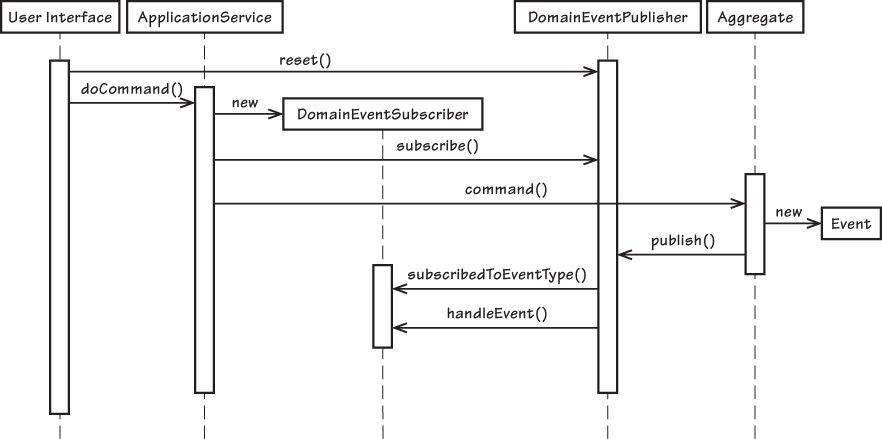
\includegraphics[width=\textwidth]{img/DomainEvent_SequenceDiagram.png}
\end{frame}

\begin{frame}[fragile]{3-1. Complete Source Code: \texttt{DomainEventPublisher}}
  \lstset{language=Java, basicstyle=\ttfamily\tiny, numbers=left, numberstyle=\tiny\color{gray}, numbersep=5pt}
\begin{lstlisting}
package com.saasovation.agilepm.domain.model;

import java.util.ArrayList;
import java.util.List;

public class DomainEventPublisher {

    @SuppressWarnings("unchecked")
    private static final ThreadLocal<List> subscribers =
            new ThreadLocal<List>();

    private static final ThreadLocal<Boolean> publishing =
            new ThreadLocal<Boolean>() {
                @Override protected Boolean initialValue() {
                    return Boolean.FALSE;
                }
            };

    public static DomainEventPublisher instance() {
        return new DomainEventPublisher();
    }
    public DomainEventPublisher() { super(); }

    @SuppressWarnings("unchecked")
    public <T> void publish(final T aDomainEvent) {
        if (publishing.get()) { // ➊ Prevent re-entrant calls
            return;
        }
        try {
            publishing.set(Boolean.TRUE);

            List<DomainEventSubscriber<T>> registeredSubscribers =
                    subscribers.get();
            if (registeredSubscribers != null) {
                Class<?> eventType = aDomainEvent.getClass();

                for (DomainEventSubscriber<T> subscriber
                        : registeredSubscribers) {

                    Class<?> subscribedTo =
                            subscriber.subscribedToEventType();

                    if (subscribedTo == eventType ||
                        subscribedTo == DomainEvent.class) {

                        subscriber.handleEvent(aDomainEvent); // ➋ Synchronous call
                    }
                }
            }
        } finally {
            publishing.set(Boolean.FALSE);
        }
    }

    public DomainEventPublisher reset() {
        if (!publishing.get()) {
            subscribers.set(null);
        }
        return this;
    }

    @SuppressWarnings("unchecked")
    public <T> void subscribe(DomainEventSubscriber<T> aSubscriber) {
        if (publishing.get()) { // ➌ Avoid modifying the list while publishing
            return;
        }
        List<DomainEventSubscriber<T>> registeredSubscribers =
                subscribers.get();
        if (registeredSubscribers == null) {
            registeredSubscribers =
                    new ArrayList<DomainEventSubscriber<T>>();
    }
    // ...
}
  \end{lstlisting}
  \begin{itemize}
    \item Each thread has its own \texttt{DomainEventPublisher} instance.
    \item \textbf{Benefit}: Natural thread isolation, avoiding concurrency issues in a web environment.
  \end{itemize}
\end{frame}

\begin{frame}[fragile]{3-3. Typical Flow of a "Single Request"}
  \lstset{language=Java, basicstyle=\ttfamily\scriptsize}
  \begin{lstlisting}
// ① Enter a Web Filter (at the start of each HTTP request)
DomainEventPublisher.instance().reset();

// ② Application Service registers subscribers
DomainEventPublisher.instance().subscribe(subscriber);

// ③ Execute Aggregate behavior → publish event
backlogItem.commitTo(aSprint); // internally calls publish(...);
  \end{lstlisting}
  \begin{itemize}
    \item `reset()` clears subscribers from the previous request.
    \item `publish()` triggers the event.
  \end{itemize}
\end{frame}

\begin{frame}[fragile]{3-4. \texttt{DomainEventSubscriber} Interface}
  \lstset{language=Java, basicstyle=\ttfamily\scriptsize}
  \begin{lstlisting}
public interface DomainEventSubscriber<T> {
    void handleEvent(T aDomainEvent);
    Class<T> subscribedToEventType();
}
  \end{lstlisting}
  \begin{itemize}
    \item `subscribedToEventType()`
      \begin{itemize}
        \item Returns the specific event class → The Publisher uses this for matching.
        \item Returning `DomainEvent.class` means "consume all events".
      \end{itemize}
    \item `handleEvent()`
      \begin{itemize}
        \item The logic should be lightweight: it should \textbf{not} modify another Aggregate. For async work (MQ / Email), write to an Outbox or schedule a task.
      \end{itemize}
  \end{itemize}
\end{frame}

\begin{frame}[fragile]{3-5. Aggregate Publishing: Revisited}
  \lstset{language=Java, basicstyle=\ttfamily\scriptsize}
  \begin{lstlisting}
public void commitTo(Sprint aSprint) {
    // ...validation and state change...
    DomainEventPublisher.instance()
        .publish(new BacklogItemCommitted(
            this.tenantId(),
            this.backlogItemId(),
            this.sprintId()));
}
  \end{lstlisting}
  \begin{itemize}
    \item First, ensure business invariants pass and state is updated ➜ then publish the event.
    \item Publishing immediately triggers all subscribers on the same thread; the transaction is only committed if successful.
  \end{itemize}
\end{frame}

\begin{frame}{✅ Summary}
  \begin{enumerate}
    \item \textbf{ThreadLocal + Synchronous Call}: Zero external dependencies, simple to test.
    \item \textbf{reset → subscribe → publish}: These three steps align with a single HTTP / gRPC request.
    \item \textbf{`publishing` flag} ensures:
      \begin{itemize}
        \item Re-entrant `publish()` calls are not allowed.
        \item `subscribe()` can only be called when not publishing, avoiding concurrent list modification.
      \end{itemize}
    \item \textbf{Subscriber Logic Limit}: Only perform reads, logging, or writes to an Outbox. \textbf{Do not directly modify other Aggregates}.
  \end{enumerate}
\end{frame}


\section{4. Outbox/Event Store \& Transactional Consistency}

\begin{frame}{Three Basic Strategies}
  \begin{itemize}
    \item<1-> \textbf{Shared Persistence Store}: Model and messages are written in the same local transaction.
      \begin{itemize}
        \item[+] Pros: Simple, strong consistency.
        \item[-] Cons: Schema pollution.
      \end{itemize}
    \item<2-> \textbf{XA Two-Phase Commit}: The model's DB and the messaging store participate in the same global transaction.
      \begin{itemize}
        \item[+] Pros: Technical separation.
        \item[-] Cons: Poor performance, limited support.
      \end{itemize}
    \item<3-> \textbf{Outbox / Event Store (★Book's Example)}: Events are first written to a local DB `events` table, then delivered by a separate forwarder.
      \begin{itemize}
        \item[+] Pros: Local transaction guarantees consistency, supports replay.
        \item[-] Cons: Requires a custom forwarder, downstream consumers need to handle deduplication.
      \end{itemize}
  \end{itemize}
\end{frame}

\begin{frame}{4-1. Why Choose Outbox / Event Store?}
  \begin{enumerate}
    \item As a message queue, publishing to various integration systems
    \item Providing pull-based notifications via REST
    \item Complete history, not just for auditing, but also for replaying
    \item Business intelligence, trend analysis, forecasting, etc.
    \item Foundation for Event Sourcing
    \item Corrections/Patches: Marking events as invalid
  \end{enumerate}
\end{frame}

\begin{frame}[fragile]{4-2. Global Subscription and Storing in Event Store}
  \lstset{language=Java, basicstyle=\ttfamily\scriptsize}
  Use AOP to intercept all Application Services and register a subscriber that "consumes all events":
  \begin{lstlisting}
@Aspect
public class IdentityAccessEventProcessor {
    @Before(
      "execution(* com.saasovation...*.*(..))")
    public void listen() {
        DomainEventPublisher
            .instance()
            .subscribe(new DomainEventSubscriber<DomainEvent>() {
                @Override
                public void handleEvent(DomainEvent aDomainEvent) {
                    store(aDomainEvent);
                }
                @Override
                public Class<DomainEvent> subscribedToEventType() {
                    return DomainEvent.class; // all events
                }
            });
    }

    private void store(DomainEvent aDomainEvent) {
        EventStore.instance().append(aDomainEvent);
    }
}
  \end{lstlisting}
\end{frame}

\begin{frame}[fragile]{4-3. \texttt{EventStore.append(...)} Source Code}
  \lstset{language=Java, basicstyle=\ttfamily\scriptsize}
  \begin{lstlisting}
package com.saasovation.identityaccess.application.eventStore;

public class EventStore {
    // Singleton access omitted...

    public void append(DomainEvent aDomainEvent) {
        String eventSerialization =
            EventStore.objectSerializer().serialize(aDomainEvent);

        StoredEvent storedEvent =
            new StoredEvent(
                aDomainEvent.getClass().getName(),
                aDomainEvent.occurredOn(),
                eventSerialization);

        this.session().save(storedEvent);
        this.setStoredEvent(storedEvent);
    }
}
  \end{lstlisting}
  `append()` first serializes the `DomainEvent`, wraps it in a `StoredEvent`, and then writes it to the database via an ORM.
\end{frame}

\begin{frame}[fragile]{4-4. \texttt{StoredEvent} Class}
  \lstset{language=Java, basicstyle=\ttfamily\scriptsize}
  \begin{lstlisting}
package com.saasovation.identityaccess.application.eventStore;

public class StoredEvent {
    private long   eventId;    // Auto-incrementing PK
    private String typeName;   // Full class name of the event
    private Date   occurredOn; // Event timestamp
    private String eventBody;  // JSON-serialized event content

    public StoredEvent(
        String aTypeName,
        Date   anOccurredOn,
        String anEventBody) {

        this.eventBody   = anEventBody;
        this.occurredOn  = anOccurredOn;
        this.typeName    = aTypeName;
    }

    // getters / no setters → immutable
}
  \end{lstlisting}
\end{frame}

\begin{frame}{Append to Event Store Sequence}
  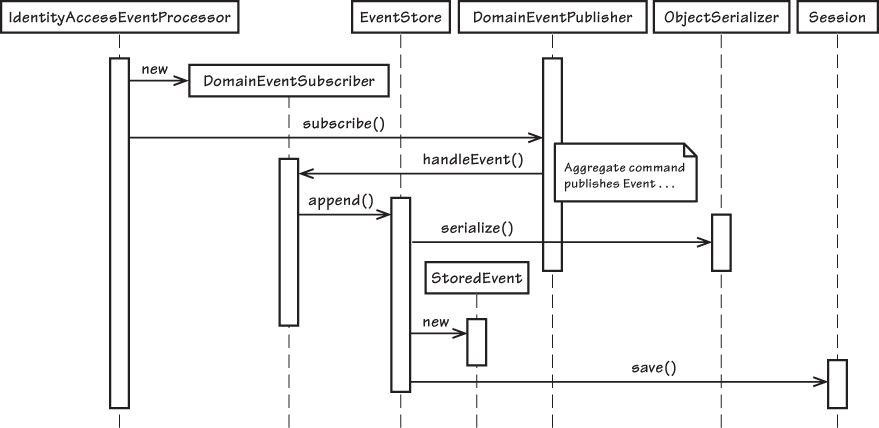
\includegraphics[width=0.9\textwidth]{img/DomainEvent_AppendToEventStore_SequenceDiagram.png}
\end{frame}

\begin{frame}[fragile]{4-5. Table DDL}
  The book uses MySQL as an example for the Event Store's table structure:
  \lstset{language=SQL, basicstyle=\ttfamily\scriptsize}
  \begin{lstlisting}
CREATE TABLE `tbl_stored_event` (
    `event_id`    int(11)      NOT NULL AUTO_INCREMENT,
    `event_body`  varchar(65000) NOT NULL,
    `occurred_on` datetime      NOT NULL,
    `type_name`   varchar(100)  NOT NULL,
    PRIMARY KEY (`event_id`)
) ENGINE=InnoDB;
  \end{lstlisting}
  This \texttt{tbl\_stored\_event} table is the implementation of the Outbox pattern.
\end{frame}

\begin{frame}{Section 4 Summary}
  \begin{itemize}
    \item \textbf{Three Consistency Strategies}: Shared DB, XA, and Outbox/Event Store; the book's example uses the Outbox pattern.
    \item \textbf{AOP Global Subscription}: `IdentityAccessEventProcessor` intercepts all AppServices, subscribes to all events, and calls `append()`.
    \item \textbf{Immutable StoredEvent}: Encapsulates serialized data, a primary key, and a timestamp.
    \item \textbf{Outbox Table DDL}: \texttt{tbl\_stored\_event} serves as the persistence area. A Forwarder then pushes its content to MQ/REST, ensuring consistency between the model and events.
  \end{itemize}
\end{frame}


\section{5. Forwarding Stored Events Across Bounded Contexts}

\begin{frame}{Architectural Pipeline}
  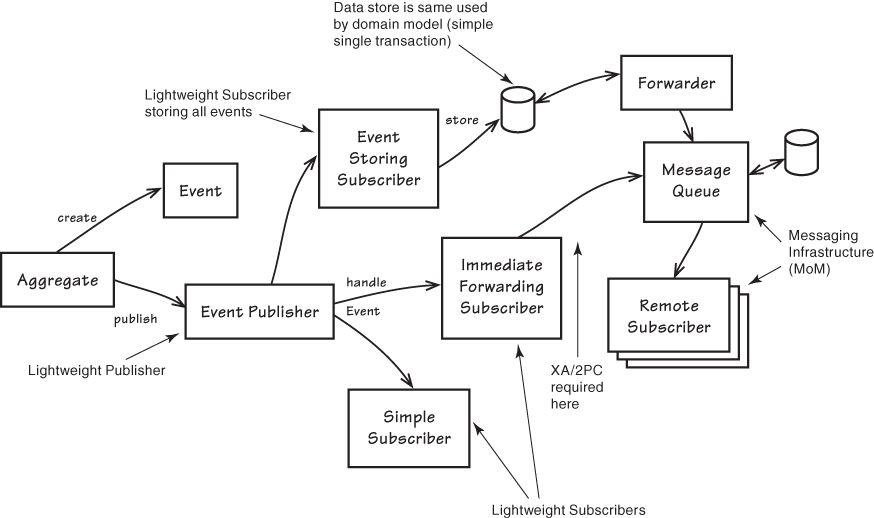
\includegraphics[width=\textwidth]{img/DomainEvent_ArchitecturePipeline.png}
\end{frame}

\begin{frame}{5-1. Architectural Style Overview}
  \begin{itemize}
    \item \textbf{Push via Middleware}:
      \begin{itemize}
        \item Use messaging middleware like RabbitMQ or ActiveMQ to \textbf{push} stored events to subscribers.
      \end{itemize}
    \item \textbf{Pull via REST}:
      \begin{itemize}
        \item Expose a notification log URI, allowing clients to periodically \textbf{pull} new events from the service.
      \end{itemize}
  \end{itemize}
\end{frame}

\begin{frame}[fragile]{5-2. \texttt{NotificationService.publishNotifications()}}
  This is the \textbf{core push process}:
  \lstset{language=Java, basicstyle=\ttfamily\tiny}
  \begin{lstlisting}
// src/.../NotificationService.java
@Transactional
public void publishNotifications() {
    // 1. Find the tracker for the last published message
    PublishedMessageTracker publishedMessageTracker =
        this.publishedMessageTracker();

    // 2. Fetch all new, unpublished StoredEvents from the Event Store
    List<Notification> notifications =
        this.listUnpublishedNotifications(
            publishedMessageTracker.mostRecentPublishedMessageId());

    // 3. Create a MessageProducer (e.g., for a RabbitMQ exchange)
    MessageProducer messageProducer = this.messageProducer();

    try {
        // 4. Push one by one
        for (Notification notification : notifications) {
            this.publish(notification, messageProducer);
        }
        // 5. Update the tracker with the ID of the last published StoredEvent
        this.trackMostRecentPublishedMessage(
            publishedMessageTracker, notifications);
    } finally {
        messageProducer.close();
    }
}
  \end{lstlisting}
\end{frame}

\begin{frame}[fragile]{5-3. Fetching Unpublished Events}
  \lstset{language=Java, basicstyle=\ttfamily\scriptsize}
  \begin{lstlisting}
// in NotificationService
protected List<Notification> listUnpublishedNotifications(
        long aMostRecentPublishedMessageId) {

    EventStore eventStore = EventStore.instance();

    List<StoredEvent> storedEvents =
      eventStore.allStoredEventsSince(aMostRecentPublishedMessageId);

    return this.notificationsFrom(storedEvents);
}
  \end{lstlisting}
  Directly calls `EventStore.allStoredEventsSince(...)` to get a sorted list of `StoredEvent`s.
\end{frame}

\begin{frame}[fragile]{5-4. Synchronously Pushing a Single Notification}
  \lstset{language=Java, basicstyle=\ttfamily\scriptsize}
  \begin{lstlisting}
// in NotificationService
protected void publish(
        Notification aNotification,
        MessageProducer aMessageProducer) {

    MessageParameters messageParameters =
      MessageParameters.durableTextParameters(
          aNotification.type(),
          Long.toString(aNotification.notificationId()),
          aNotification.occurredOn());

    String notification = objectSerializer().serialize(aNotification);

    aMessageProducer.send(notification, messageParameters);
}
  \end{lstlisting}
  Header used for deduplication and quick filtering, `notificationId` supports deduplication.
\end{frame}

\begin{frame}[fragile]{5-5. Establishing/Reconnecting a RabbitMQ Producer}
  \lstset{language=Java, basicstyle=\ttfamily\scriptsize}
  \begin{lstlisting}
// in NotificationService
private MessageProducer messageProducer() {
    Exchange exchange = Exchange.fanOutInstance(
        ConnectionSettings.instance(),
        EXCHANGE_NAME,
        true);

    return MessageProducer.instance(exchange);
}
  \end{lstlisting}
  Rebuilds the connection each time to avoid long connection errors.
\end{frame}

\begin{frame}[fragile]{5-6. Periodically Triggering the Push}
  The book uses \textbf{JMX TimerMBean} to periodically trigger:
  \lstset{language=Java, basicstyle=\ttfamily\tiny}
  \begin{lstlisting}
// Register MBean listener somewhere
mbeanServer.addNotificationListener(
    timer.getObjectName(),
    new NotificationListener() {
        @Override
        public void handleNotification(
                Notification aTimerNotification,
                Object aHandback) {

            ApplicationServiceRegistry
                .notificationService()
                .publishNotifications();
        }
    },
    null,
    null);
  \end{lstlisting}
\end{frame}

\begin{frame}[fragile]{5-7. RESTful Pull Style (Brief)}
  \lstset{language=Java, basicstyle=\ttfamily\scriptsize}
  \begin{lstlisting}
@Path("/notifications")
public class NotificationResource {
    @GET @Produces(...)
    public Response getCurrentNotificationLog() {
        NotificationLog log =
          notificationService.currentNotificationLog();
        // Convert to REST DTO and return JSON
    }
    @GET @Path("{id}") ...
    public Response getNotificationLog(...) { ... }
}
  \end{lstlisting}
  Clients can periodically poll `/notifications` to pull the latest events.
\end{frame}

\begin{frame}{5-8. Summary}
  \begin{itemize}
    \item \textbf{Push}: `NotificationService` batch-pushes StoredEvents to RabbitMQ, using a Tracker to ensure exactly-once logic.
    \item \textbf{Pull}: Provide current \& historical NotificationLogs via a JAX-RS Resource.
    \item \textbf{Latency Tolerance}: The event stream is eventually consistent and can tolerate delays.
  \end{itemize}
\end{frame}

\begin{frame}{Notification Log Pagination}
  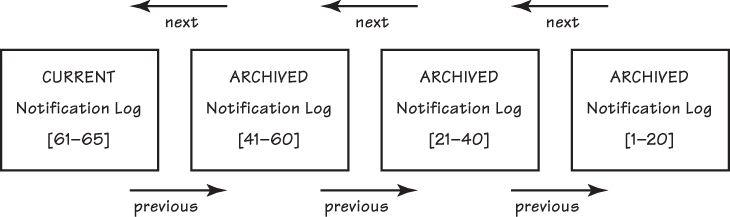
\includegraphics[width=0.8\textwidth]{img/DomainEvent_NotificationLog_Pagination.png}
\end{frame}


\section{6. Common Pitfalls \& Testing Strategies}

\begin{frame}{Common Pitfalls}
  \begin{itemize}
    \item \textbf{Event handler modifies a second Aggregate}: Violates the "one transaction, one Aggregate" rule.
    \item \textbf{Failure to reset subscribers leads to leftovers}: The `ThreadLocal` subscriber list is not `reset()` at the start of a request.
    \item \textbf{Nested publishes are ignored}: The `publishing` flag skips subsequent `publish()` calls within a handler.
    \item \textbf{Lack of idempotency and deduplication}: A unique ID is needed for deduplication in cross-system communication.
  \end{itemize}
\end{frame}

\begin{frame}[fragile]{Testing Strategy (1) - Publisher/Subscriber Unit Test}
  \lstset{language=Java, basicstyle=\ttfamily\tiny}
  \begin{lstlisting}
public class DomainEventPublisherTest {
  @Before
  public void setUp() {
    DomainEventPublisher.instance().reset();
  }

  @Test
  public void whenPublish_thenSubscriberReceivesEvent() {
    AtomicReference<MyDomainEvent> received = new AtomicReference<>();
    DomainEventPublisher.instance().subscribe(
      new DomainEventSubscriber<MyDomainEvent>() {
        public void handleEvent(MyDomainEvent e) { received.set(e); }
        public Class<MyDomainEvent> subscribedToEventType() { 
          return MyDomainEvent.class; 
        }
      }
    );

    MyDomainEvent evt = new MyDomainEvent(...);
    DomainEventPublisher.instance().publish(evt);
    assertSame(evt, received.get());
  }
}
  \end{lstlisting}
\end{frame}

\begin{frame}{Testing Strategy (2) - Other Strategies}
  \begin{enumerate}
    \item \textbf{Event Store (Outbox) Test}: Verify that serialization, ordering, and persistence are correct.
    \item \textbf{Modeling Tests}: Test domain object behavior and invariants.
    \item \textbf{Mocked Notification Forwarder Test}: Mock the `MessageProducer` to verify that events are `send()` and the tracker is updated.
    \item \textbf{Idempotent Consumer Test}: Simulate sending the same event multiple times and assert that the handling logic is executed only once.
  \end{enumerate}
\end{frame}

\begin{frame}{Conclusion}
  The above are common pitfalls and corresponding testing strategies for implementing Domain Events. They help you adhere to the single-Aggregate rule while ensuring the reliability and testability of your event mechanism.
  \vfill
\end{frame}


\appendix
\section{Appendix: Deeper Dive}

\begin{frame}{A. Event Identity}
  \begin{enumerate}
    \item \textbf{When is it needed?}: For deduplication across systems, comparison, or when accessed as an Aggregate.
    \item \textbf{Identity from event attributes}: Event name + Aggregate ID(s) + `occurredOn` timestamp is usually sufficient.
    \item \textbf{Formally generating a unique ID}: If attributes are insufficient, a UUID can be assigned.
    \item \textbf{Provided by message middleware}: Many MQs provide a unique message ID in the header.
    \item \textbf{equals()/hashCode()}: Only need to be implemented if the event is stored as an Aggregate.
  \end{enumerate}
\end{frame}

\begin{frame}[fragile]{B. Modeling Events as Aggregates}
  When an event is created directly from a client request, it can be modeled as an Aggregate.
  \begin{itemize}
    \item \textbf{Immutable}: All state is injected during construction.
    \item \textbf{Unique Identity}: A specially generated ID.
    \item \textbf{Independent Storage}: First saved to a Repository, then published.
  \end{itemize}
  \lstset{language=Java, basicstyle=\ttfamily\tiny}
  \begin{lstlisting}
public class ClientTriggeredEvent implements DomainEvent {
    private final EventId       eventId;
    private final Date          occurredOn;
    private final ImportantData data;
    // Constructor fills all fields at once → immutable
    // getters...
}

public class EventCreationService {
    public void createAndPublish(ImportantData d) {
        ClientTriggeredEvent e =
          new ClientTriggeredEvent(new EventId(), new Date(), d);
        this.eventRepository.save(e); // Never delete
        this.messagePublisher.publish(e); // Outbox or XA
    }
}
  \end{lstlisting}
\end{frame}

\begin{frame}{C. Whiteboard Time Exercise}
  \begin{itemize}
    \item \textbf{List existing but uncaptured events}:
      \begin{itemize}
        \item User login failure, automatic order cancellation on timeout...
      \end{itemize}
    \item \textbf{Consider model improvements}:
      \begin{itemize}
        \item Can turning them into explicit Domain Events replace complex batch queries?
      \end{itemize}
    \item \textbf{Focus on dependencies}:
      \begin{itemize}
        \item Pay attention to scenarios that cross Aggregates and require eventual consistency.
      \end{itemize}
    \item \textbf{Keep event behavior side-effect free}:
      \begin{itemize}
        \item Only perform side-effect-free queries and data encapsulation.
      \end{itemize}
  \end{itemize}
\end{frame}

\end{document}
